\chapter{Theoretical Background}
\label{chap:background}

\section{Video Coding}

A problem of uncompressed videos (RAW) have been the storage and transmission
due to the big number of bits that it contains. For this reason, the use of
compression techniques is required for reducing the numbers of bits that
represents the video. The video coding have advantage of three types of
redundancy present in a video \cite{motion}:

\begin{itemize}
  \item \textbf{Statistical redundancy:} refers to the high spatial correlation
  between pixels in a frame and the high temporal correlation between
  co-localizated pixels in consecutive frames.
  \item \textbf{Psychovisual redundancy:} due to the limitations and
  characteristic of the human visual system, the not distinguished information
  is removed.
  \item \textbf{Coding Redundancy:} is produced by the repetition of symbols
  that represent the video information.
\end{itemize}

Video coding standards implement a set of tools for exploiting this redundancies
of video. Figure \ref{codec} presents a block diagram of a video coding
standard, which have two main module, the encoder and the decoder.

\begin{figure}[!h]
\centering
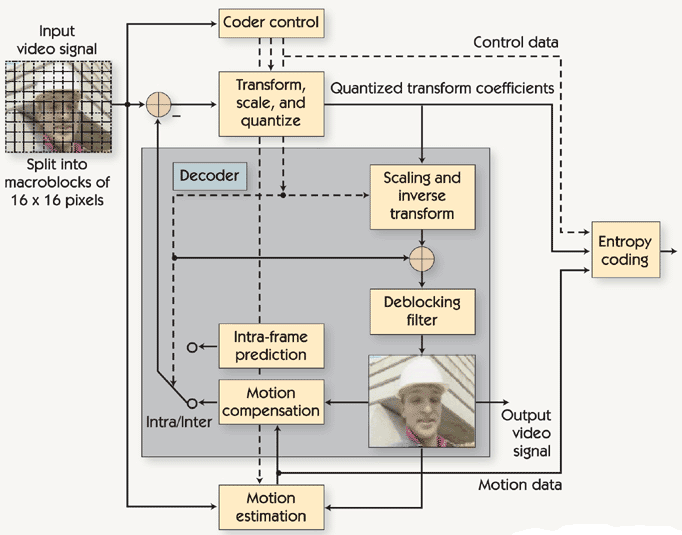
\includegraphics[width=0.6\textwidth]{images/codec.png}
\caption[Block diagram of a video coding standard]{Block diagram of a video coding standard
\scriptsize{\textbf{Source:}
\url{http://www.eetimes.com/document.asp?doc_id=1272639}}}
\label{codec}
\end{figure}

The video encoders consist of three main elements, which exploit each 
redundancy presents in  a video:

\begin{itemize}
	\item The \textbf{predictor} performs a intra-frame prediction for
	exploiting the spatial correlation and  a inter-frame-predicition for
	exploiting the temporal correlation.
	\item The \textbf{quantizer} reduces the accuracy of representations generated
	by the predictor through a fidelity criterion for eliminating the psychovisual
	redundancy.
	\item The \textbf{entropy encoder} reduces the number of symbols needded for
	representing the video taking advantange of the similarity of resulting symbols
	in the quantizer.
\end{itemize}

The video decoders perform the iverse process of each component for
reconstructing the coded information. In the reconstruction process is presented
a loss of information because the de-quantization process don't recover the
original information transformed in the encoder.

\section{Sparse Representation}

Loss information in the video coding is related to two suppositions: the fisrt
is teh imperfection of the HVS (sensitivity) an the second is related to
specific properties of the signals in certain transform domain. The objective of
sparse representation is reconstruct a signal using a small set of signal
samples \cite{compressive}. 

Let a signal $\boldsymbol{x} \in \mathbb{R}^N$. Given a orthonormal matrix
$\boldsymbol{B} \in \mathbb{R}^{N \times N}$, where its columns are the base
elements $ \{\boldsymbol{b}_i\}_{i=1}^N$, $\boldsymbol{x}$ can be represented
in terms of this base as:

\begin{center}
\begin{equation}
\boldsymbol{x}=\sum \limits_{i=1}^{N} \boldsymbol{\alpha}_i \boldsymbol{b}_i
\end{equation}
\end{center}

where $\boldsymbol{\alpha}$ is a coefficients vector and $\boldsymbol{b}_i$ are
the atoms of dictionary \cite{sparsity}. These coefficients are given by
$\alpha_i = \boldsymbol{x} \boldsymbol{b}_i^T$. If the number of non-zero
coefficients in $\boldsymbol{x}$ is $K\ll N$, the base $\boldsymbol{b}$
provides a K-sparse representation of $\boldsymbol{x}$. Ths sparse
representation of a $\boldsymbol{\alpha}$ vector  is related to $||\alpha||_0 =
K$ where $||.||_p$ indicates the  $\ell_p$-norm defined as:

\begin{equation}
||\boldsymbol{\alpha}||_p = \left(\sum\limits_{i=1}^{n} |\alpha_i|^p \right)^\frac{1}{p}
\end{equation}

and $||\alpha||_0$ is the $\ell_0$-norm, which indicates the number of
non-zero elements in the vector, and is defined as:

\begin{equation}
||\boldsymbol{\alpha}||_0 = \lim_{p \to 0} ||\alpha||_p^p=\lim_{p \to 0} \sum_i |\alpha_i|^p
\end{equation} 

Generally, the real world signals are not exactly sparse in a orthogonal base,
instead, these are compressibles. A signal is compressible if the
coefficents magnitude, in a decreasing order, present decay in the power law,
such as:

\begin{equation}
|\alpha|_{(n)} \leq C n^{-s}\;,\quad s=1,2 \ldots
\end{equation}

where $L$ is the term of a lineal combination of elements that approximate to
$\boldsymbol{x}$.

\subsection{Incoherent Sampling}

A set of random samples selected from the signal $\boldsymbol{x}$ are used for
constructing a $\boldsymbol{\phi} \in \mathbb{R}^{M \times N}$ matrix, such as:

\begin{equation}
\boldsymbol{y} = \boldsymbol{\phi x}
\end{equation}

where 

Un conjunto de muestras aleatorias seleccionadas desde la se\~nal $\boldsymbol{x}$ son usadas para construir una matriz $\boldsymbol{\phi} \in \mathbb{R}^{M \times N}$ tal que:
\begin{equation}
\boldsymbol{y} = \boldsymbol{\phi x}
\end{equation}
donde $\boldsymbol{y}$ es un vector $M\times 1$ de medidas compresivas.  Para reconstruir $\boldsymbol{x}$ desde $\boldsymbol{y}$, $\boldsymbol{x}$ debe ser disperso en un dominio transformado (definido por la matriz de base ortogonal $\boldsymbol{B}$), tal que:
\begin{equation}
\boldsymbol{y}=\boldsymbol{\phi B \alpha}= \boldsymbol{D\alpha}
\end{equation}
La incoherencia est\'a relacionada con la propiedad de la se\~nales que tiene representaci\'on dispersa en un dominio transformado $\boldsymbol{\psi}$, las cuales deben ser densas en el dominio donde se realiz\'o la adquisici\'on \cite{compressive}. La coherencia entre una base sensada $\boldsymbol{\phi}$  y una base de representaci\'on $\boldsymbol{\psi}$ est\'a dada por: 

\begin{equation}
\mu(\boldsymbol{\phi},\boldsymbol{B})= \sqrt{N} \max_{1 \leq j, j \leq N} | \boldsymbol{\varphi}_i,\boldsymbol{b}_j|, \quad 1\leq \mu(\boldsymbol{\phi},\boldsymbol{B}) \sqrt{N}
\end{equation}
Si la coherencia es baja, un n\'umero de muestras aleatorias para reconstruir la se\~nal es peque\~no porque cada fila de $\boldsymbol{\phi}$ se extiende en el dominio $\boldsymbol{B}$.

\subsection{Propiedad Isom\'etrica Restringida (RIP)}

Esta propiedad ayuda a determinar si la matriz $\boldsymbol{D}$ es  buena para realizar CS. Una matriz $\boldsymbol{D}$ satisface la RIP, si por cada $K = 1,2, \ldots, N$, la constante isom\'etrica $\delta_K$ de la matriz $\boldsymbol{D}$ es el n\'umero m\'as peque\~no, tal que: 
\begin{equation}
(1-\delta_K)||\boldsymbol{x}||_2^2 \leq ||\boldsymbol{Dx}||^2_2 \leq (1+\delta_K)||\boldsymbol{x}||^2_2
\end{equation}
para todos los vectores K-dispersos de $\boldsymbol{x}$. Est\'a propiedad es equivalente a decir que todos los $K$ subconjuntos tomados de las columnas pertenecientes a $\boldsymbol{D}$ son casi ortogonales y los vectores K-dispersos no se encuentran en el espacio nulo de $\boldsymbol{D}$.

\subsection{Optimizaciones Num\'ericas}

Un sistema de ecuaciones lineales con una matriz $\boldsymbol{D} \in \mathbb{R}^{M \times N}$ representa un sistema de ecuaciones indeterminado que puede tener infinitas soluciones. El m\'etodo para resolver este sistema y hallar la representaci\'on dispersa de la se\~nal es encontrar la norma m\'inima mediante un proceso de optimizaci\'on, tal que: 
\begin{equation}
\min||\boldsymbol{\alpha^\prime}||_0 \quad \textrm{subject to} \; \boldsymbol{x} = \boldsymbol{D \alpha^\prime}
\end{equation}
Aunque solucionando este problema de optimizaci\'on se puede hallar directamente la representaci\'on dispersa, es un problema NP-Hard porque requiere una b\'usqueda combinatoria exhaustiva. En algunos casos, es usada la norma $\ell_1$ y $\ell_2$ para aproximar la soluci\'on dispersa. \\


El proceso de CS es resumido en la Figura \ref{fig:compressive}. Una vez es conseguida una soluci\'on dispersa, la se\~nal puede ser recosntruida en base a un vector con una gran cantidad de coeficientes igual a cero y un diccionario $\boldsymbol{D}=\boldsymbol{\phi B}$.
\begin{figure}[!h]
\centering
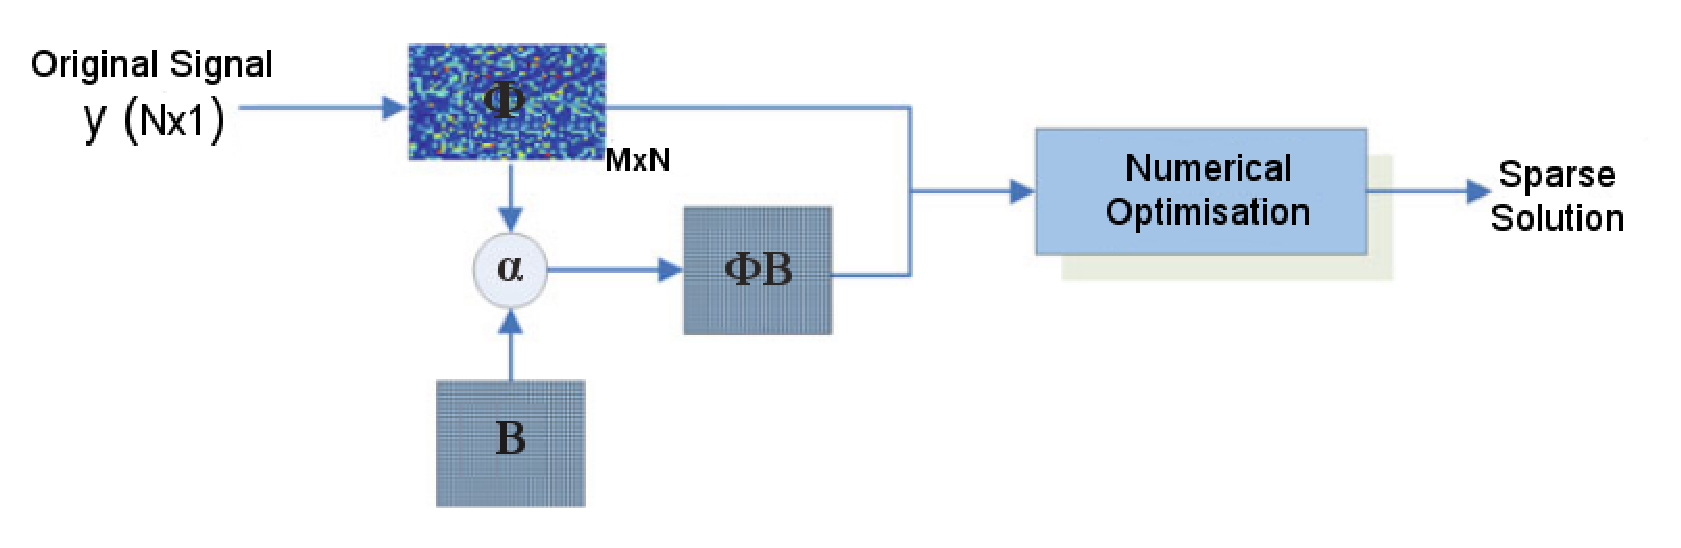
\includegraphics[width=\textwidth]{images/sparse.eps}
\caption[Proceso de \textit{Compressed sensing}]{Proceso de \textit{Compressed sensing} \cite{compressive}}
\label{fig:compressive}
\end{figure}











